\textbf{Detección y Clasificación de Objetos}: Ideal para tareas de visión artificial, la Jetson Nano utiliza frameworks como TensorFlow y PyTorch.

\begin{figure}[H]
  \centering
  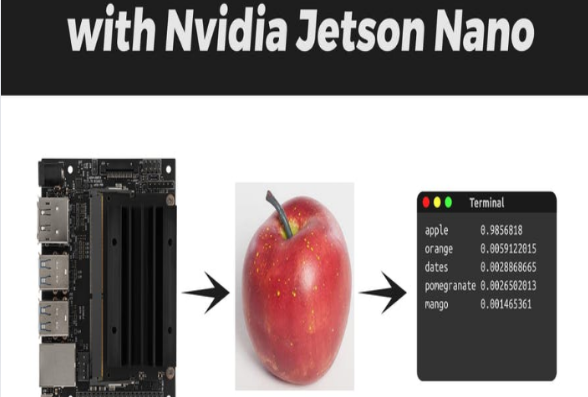
\includegraphics[scale = 0.7]{Imagenes/clasificacion_objetos.png}
  \caption{Detección y extracción de datos}{Fuente: Internet}
\end{figure}

\textbf{Robots Autónomos}: Su capacidad de procesamiento en tiempo real permite a los robots interpretar su entorno, identificar objetos.

\begin{figure}[H]
  \centering
  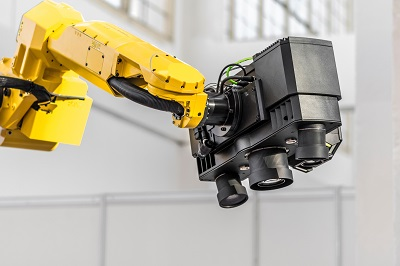
\includegraphics[scale = 1]{Imagenes/jetson_surveillance.jpg}
  \caption{Brazo robot de vigilancia}{Fuente: Internet}
\end{figure}

\textbf{Aplicaciones Médicas}: En el ámbito de la salud, la Jetson Nano facilita el análisis de imágenes médicas.

\begin{figure}[H]
  \centering
  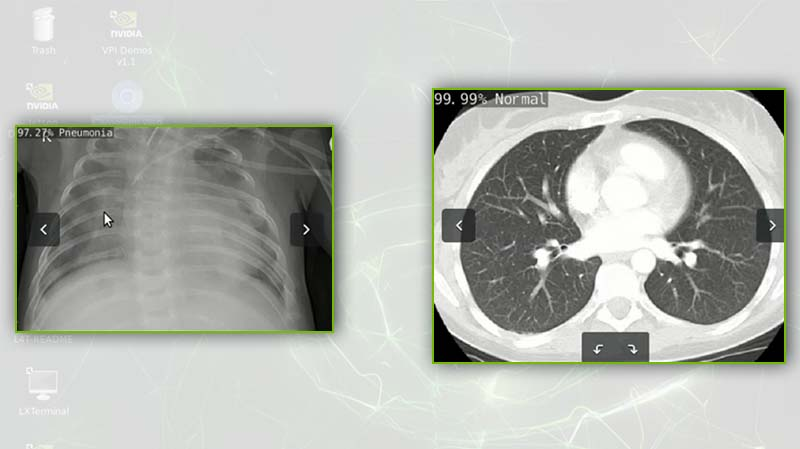
\includegraphics[scale = 0.5]{Imagenes/healthcare.jpg}
  \caption{Análisis de imágenes}{Fuente: Internet}
\end{figure}

\textbf{Proyectos de IoT}: Ideal para aplicaciones de Internet de las Cosas, donde se necesita una toma de decisiones rápida sin depender de la nube, como en el monitoreo ambiental.

\begin{figure}[H]
  \centering
  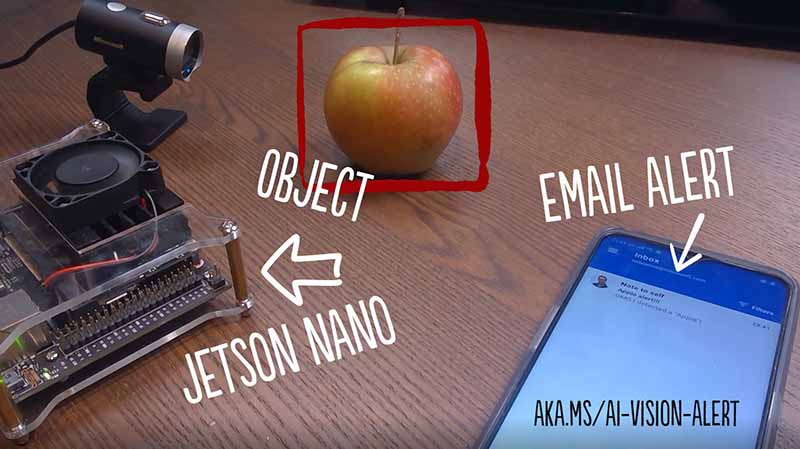
\includegraphics[scale = 0.5]{Imagenes/IoT.jpg}
  \caption{Sistema IoT}{Fuente: Internet}
\end{figure}